\documentclass[11pt,a4paper]{article}
% Reuse the visual language of the first exercise session.
\usepackage[margin=18mm,headheight=24pt]{geometry}
\usepackage[T1]{fontenc}
\usepackage[english]{babel}
\usepackage{lmodern}
\usepackage{microtype}
\usepackage{amsmath,amssymb}
\usepackage{siunitx}
\usepackage{tikz}
\usetikzlibrary{arrows.meta,calc,angles,quotes}
\usepackage{enumitem}
\usepackage{xcolor}
\usepackage{fancyhdr}
\usepackage{lastpage}
\usepackage[hidelinks]{hyperref}

\definecolor{VectorGreen}{HTML}{174A38}
\definecolor{VectorAccent}{HTML}{216343}
\definecolor{VectorMint}{HTML}{E2F0E5}
\definecolor{VectorCoral}{HTML}{C45136}
\definecolor{VectorInk}{HTML}{203B31}
\definecolor{VectorMuted}{HTML}{5F7468}

\color{VectorInk}
\setlength{\parindent}{0pt}
\setlength{\parskip}{0.55em}
\setlist[enumerate]{leftmargin=*,itemsep=0.45em,topsep=0.35em}
\sisetup{per-mode=symbol}

\pagestyle{fancy}
\fancyhf{}
\lhead{\textcolor{VectorMuted}{Vectors · Exercise session}}
\rhead{\textcolor{VectorMuted}{Addition and subtraction}}
\cfoot{\textcolor{VectorMuted}{\thepage\ / \pageref*{LastPage}}}
\renewcommand{\headrulewidth}{0.4pt}
\renewcommand{\headrule}{\hbox to\headwidth{\color{VectorMint}\leaders\hrule height \headrulewidth\hfill}}

\newcommand{\sessiontitle}[2]{%
  {\color{VectorGreen}\fontsize{25}{29}\selectfont\bfseries #1\par}
  \vspace{0.2em}
  {\color{VectorMuted}\large #2\par}
  \vspace{0.55em}
  {\color{VectorAccent}\rule{\textwidth}{1.5pt}}
}

\newcommand{\problemheading}[2]{%
  {\color{VectorAccent}\small\bfseries\MakeUppercase{Problem #1}}\par
  {\color{VectorGreen}\LARGE\bfseries #2}\par
  \vspace{0.25em}
}

\newcommand{\prediction}[1]{%
  \begin{center}
  \colorbox{VectorMint}{\parbox{0.92\linewidth}{\textbf{Predict before calculating.} #1}}
  \end{center}
}

\newcommand{\checkpoint}[1]{%
  \begin{center}
  \fcolorbox{VectorAccent}{white}{\parbox{0.91\linewidth}{\textbf{Reasoning checkpoint.} #1}}
  \end{center}
}

\newcommand{\worklines}[1]{%
  \par\vspace{0.25em}
  {\color{VectorMuted}\small\textit{Working and explanation}}\par
  \foreach \n in {1,...,#1}{\vspace{0.54cm}\noindent\textcolor{VectorMint}{\rule{\linewidth}{0.35pt}}\par}
}

\newcommand{\answerbox}[1]{%
  \begin{center}
  \colorbox{VectorMint}{\parbox{0.92\linewidth}{\textbf{Answer.} #1}}
  \end{center}
}

\lhead{\textcolor{VectorMuted}{Motion · Exercise session 2}}
\rhead{\textcolor{VectorMuted}{Constant acceleration}}


\begin{document}
\sessiontitle{Motion hides in the timing}{Exercise session 2 · Read the picture, find the unknowns}

Problems 1 and 2 are required; Problem 3 is an optional challenge.

\problemheading{1}{Three snapshots, one missing story}

A robot is moving. You have three camera snapshots. The same constant acceleration throughout. \textbf{Reconstruct the motion}:$\vec v_0=\ ?,\vec a=\ ?$

\begin{center}
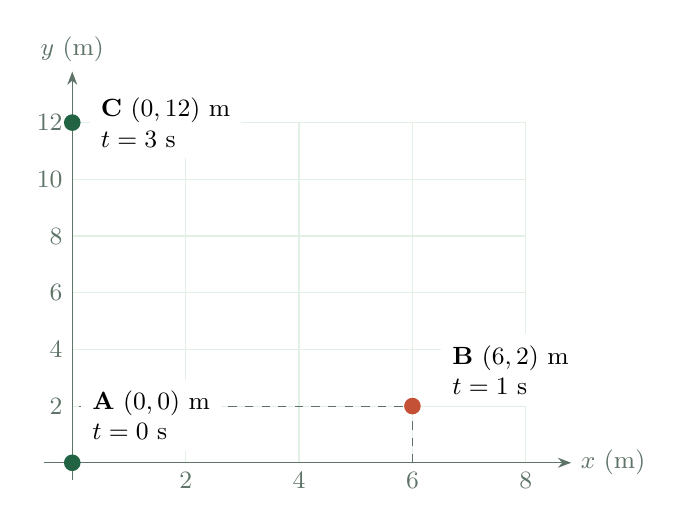
\begin{tikzpicture}[>=Stealth,x=0.72cm,y=0.36cm,font=\small]
  \draw[step=2,VectorMint,thin] (0,0) grid (8,12);
  \draw[->,VectorMuted] (-0.5,0)--(8.8,0) node[right] {$x$ (m)};
  \draw[->,VectorMuted] (0,-0.6)--(0,13.8) node[above] {$y$ (m)};
  \foreach \x in {2,4,6,8}{\node[below,VectorMuted] at (\x,0) {\x};}
  \foreach \y in {2,4,6,8,10,12}{\node[left,VectorMuted] at (0,\y) {\y};}
  \draw[dashed,VectorMuted] (6,0)--(6,2)--(0,2);
  \fill[VectorAccent] (0,0) circle (3pt);
  \node[above right,fill=white,inner sep=4pt,align=left] at (0.15,0.4)
    {\textbf{A} $(0,0)$ m\\$t=0$ s};
  \fill[VectorCoral] (6,2) circle (3pt);
  \node[above right,fill=white,inner sep=4pt,align=left] at (6.5,2)
    {\textbf{B} $(6,2)$ m\\$t=1$ s};
  \fill[VectorAccent] (0,12) circle (3pt);
  \node[right,fill=white,inner sep=4pt,align=left] at (0.3,12)
    {\textbf{C} $(0,12)$ m\\$t=3$ s};
\end{tikzpicture}

\vspace{0.5em}
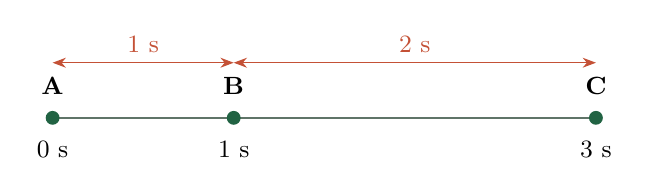
\begin{tikzpicture}[>=Stealth,x=2.3cm,font=\small]
  \draw[thick,VectorMuted] (0,0)--(3,0);
  \foreach \t/\name in {0/A,1/B,3/C}{
    \fill[VectorAccent] (\t,0) circle (2.5pt);
    \node[above=5pt] at (\t,0) {\textbf{\name}};
    \node[below=5pt] at (\t,0) {$\t$ s};
  }
  \draw[<->,VectorCoral] (0,0.7)--node[above] {1 s}(1,0.7);
  \draw[<->,VectorCoral] (1,0.7)--node[above] {2 s}(3,0.7);
\end{tikzpicture}
\end{center}

\begin{enumerate}[label=\alph*)]
  \item Find the initial velocity $\vec v_0$ and acceleration $\vec a$.
  \item When is the robot farthest right? Is it stopped at that instant?
  \item Find its average velocity from A to C.
\end{enumerate}

\worklines{4}

\clearpage
\problemheading{2}{A throw through a moving window}

Choose the upward launch component $u$ so the ball clears the moving window.

\begin{center}
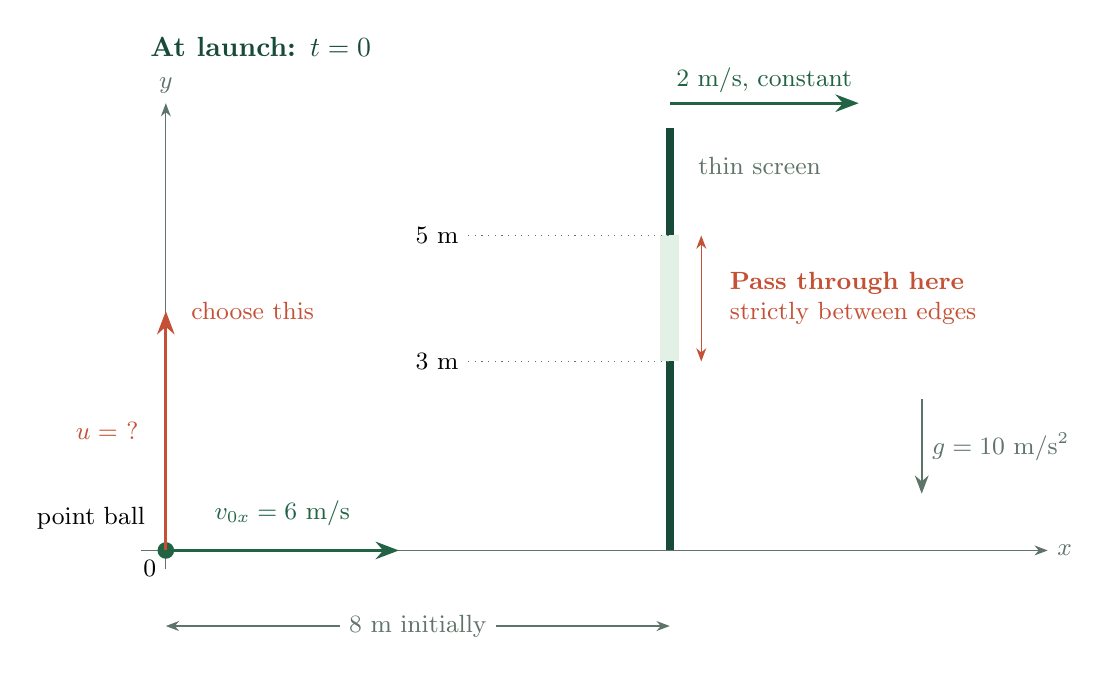
\begin{tikzpicture}[>=Stealth,x=0.8cm,y=0.8cm,font=\small]
  \node[anchor=west,VectorGreen,font=\bfseries] at (-0.4,8.0) {At launch: $t=0$};
  \draw[->,VectorMuted] (-0.4,0)--(14,0) node[right] {$x$};
  \draw[->,VectorMuted] (0,-0.3)--(0,7.1) node[above] {$y$};
  \node[below left] at (0,0) {$0$};
  \fill[VectorAccent] (0,0) circle (3pt);
  \node[above left=4pt,align=center] at (0,0) {point ball};
  \draw[->,very thick,VectorAccent] (0,0)--(3.7,0)
    node[midway,above=5pt] {$v_{0x}=6$ m/s};
  \draw[->,very thick,VectorCoral] (0,0)--(0,3.8)
    node[midway,left=6pt] {$u=\ ?$};
  \node[VectorCoral,anchor=west] at (0.25,3.8) {choose this};
  \fill[VectorMint] (7.85,3) rectangle (8.15,5);
  \draw[line width=2.8pt,VectorGreen] (8,0)--(8,3);
  \draw[line width=2.8pt,VectorGreen] (8,5)--(8,6.7);
  \draw[dotted,VectorMuted] (4.8,3)--(8,3);
  \draw[dotted,VectorMuted] (4.8,5)--(8,5);
  \node[left] at (4.8,3) {3 m};
  \node[left] at (4.8,5) {5 m};
  \draw[<->,VectorCoral] (8.5,3)--(8.5,5);
  \node[anchor=west,align=left,VectorCoral] at (8.8,4)
    {\textbf{Pass through here}\\strictly between edges};
  \draw[->,very thick,VectorAccent] (8,7.1)--(11,7.1)
    node[midway,above] {2 m/s, constant};
  \node[anchor=west,VectorMuted] at (8.3,6.1) {thin screen};
  \draw[<->,VectorMuted] (0,-1.2)--node[fill=white] {8 m initially}(8,-1.2);
  \draw[->,thick,VectorMuted] (12,2.4)--(12,0.9)
    node[midway,right] {$g=10$ m/s$^2$};
\end{tikzpicture}

{\small\color{VectorMuted}No air resistance. The screen keeps moving during the flight.}
\end{center}

\begin{enumerate}[label=\alph*)]
  \item When does the ball reach the screen?
  \item What range of $u$ lets it pass through the window?
  \item To pass through the centre, what must $u$ be? Is the ball rising or falling there?
\end{enumerate}

\worklines{7}

\clearpage
\problemheading{3}{The slowest possible interception}
{\color{VectorCoral}\bfseries Optional · Difficult}

Release the target and launch the ball at the same instant. Find the slowest successful launch. (How would you choose the coordinate system so that motion is simplest?)

\begin{center}
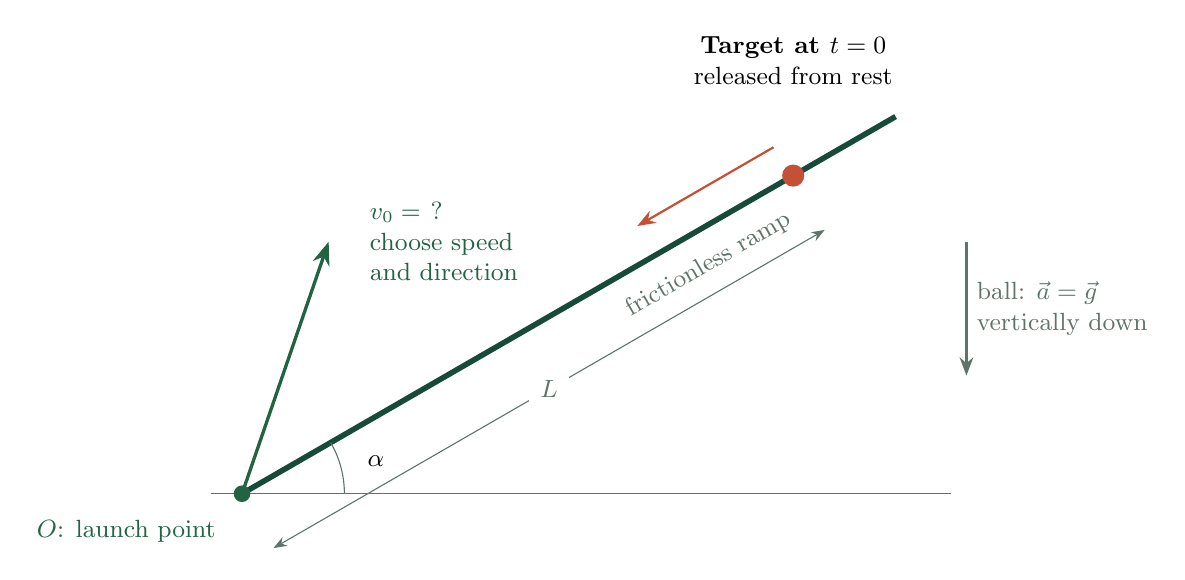
\begin{tikzpicture}[>=Stealth,x=1cm,y=1cm,font=\small]
  \draw[VectorMuted] (-0.4,0)--(9,0);
  \draw[line width=2pt,VectorGreen] (0,0)--(8.3,4.79);
  \node[rotate=30,below=5pt,VectorMuted] at (5.7,3.29) {frictionless ramp};
  \draw[VectorMuted] (1.3,0) arc (0:30:1.3);
  \node at (1.7,0.42) {$\alpha$};
  \fill[VectorAccent] (0,0) circle (3pt) node[below left=6pt] {$O$: launch point};
  \fill[VectorCoral] (7,4.04) circle (4pt);
  \node[align=center] at (7,5.5)
    {\textbf{Target at $t=0$}\\released from rest};
  \draw[->,thick,VectorCoral] (6.75,4.4)--(5.02,3.4);
  % \node[align=center,VectorCoral] at (3.8,4.7)
  %   {$a_T=g\sin\alpha$\\down the ramp};
  \draw[<->,VectorMuted] (0.4,-0.69)--node[midway,fill=white,inner sep=4pt] {$L$}(7.4,3.35);
  \draw[->,very thick,VectorAccent] (0,0)--(1.1,3.2);
  \node[anchor=west,align=left,VectorAccent] at (1.5,3.2)
    {\textbf{$v_0=\ ?$}\\choose speed\\and direction};
  \draw[->,thick,VectorMuted] (9.2,3.2)--(9.2,1.5)
    node[midway,right,align=left] {ball: $\vec a=\vec g$\\vertically down};
  % \draw[->,VectorMuted] (-1.1,2.0)--(-0.06,2.6) node[right] {$s$};
  % \draw[->,VectorMuted] (-1.1,2.0)--(-1.7,3.04) node[above] {$n$};
  % \node[below=4pt,align=center,VectorMuted] at (-1.1,2.0) {ramp axes};
\end{tikzpicture}

\colorbox{VectorMint}{\parbox{0.90\linewidth}{\centering
\textbf{Successful interception}\par
Meet on the ramp at $t>0$, before the target reaches $O$.\par
Both objects are points. $0<\alpha<90^\circ$. No air resistance.}}
\end{center}

\begin{enumerate}[label=\alph*)]
  \item For a meeting at time $t$, find the launch components $v_{0s}$ and $v_{0n}$, and the allowed range of $t$.
  \item Ignoring the deadline at $O$, find the least launch speed and its direction.\par
    {\small\color{VectorMuted}Hint: use $(A-B)^2\ge0$.}
  \item For which ramp angles is that minimum possible? For the others, find the speed that can be approached but never attained.
\end{enumerate}

\worklines{4}
\end{document}
